%-------------------------------------------------------------------------------
%	Packages and other Document configurations
%-------------------------------------------------------------------------------
\documentclass[a4paper,11pt]{article}\usepackage[]{graphicx}\usepackage[]{xcolor}
% maxwidth is the original width if it is less than linewidth
% otherwise use linewidth (to make sure the graphics do not exceed the margin)
\makeatletter
\def\maxwidth{ %
  \ifdim\Gin@nat@width>\linewidth
    \linewidth
  \else
    \Gin@nat@width
  \fi
}
\makeatother

\definecolor{fgcolor}{rgb}{0.345, 0.345, 0.345}
\newcommand{\hlnum}[1]{\textcolor[rgb]{0.686,0.059,0.569}{#1}}%
\newcommand{\hlstr}[1]{\textcolor[rgb]{0.192,0.494,0.8}{#1}}%
\newcommand{\hlcom}[1]{\textcolor[rgb]{0.678,0.584,0.686}{\textit{#1}}}%
\newcommand{\hlopt}[1]{\textcolor[rgb]{0,0,0}{#1}}%
\newcommand{\hlstd}[1]{\textcolor[rgb]{0.345,0.345,0.345}{#1}}%
\newcommand{\hlkwa}[1]{\textcolor[rgb]{0.161,0.373,0.58}{\textbf{#1}}}%
\newcommand{\hlkwb}[1]{\textcolor[rgb]{0.69,0.353,0.396}{#1}}%
\newcommand{\hlkwc}[1]{\textcolor[rgb]{0.333,0.667,0.333}{#1}}%
\newcommand{\hlkwd}[1]{\textcolor[rgb]{0.737,0.353,0.396}{\textbf{#1}}}%
\let\hlipl\hlkwb

\usepackage{framed}
\makeatletter
\newenvironment{kframe}{%
 \def\at@end@of@kframe{}%
 \ifinner\ifhmode%
  \def\at@end@of@kframe{\end{minipage}}%
  \begin{minipage}{\columnwidth}%
 \fi\fi%
 \def\FrameCommand##1{\hskip\@totalleftmargin \hskip-\fboxsep
 \colorbox{shadecolor}{##1}\hskip-\fboxsep
     % There is no \\@totalrightmargin, so:
     \hskip-\linewidth \hskip-\@totalleftmargin \hskip\columnwidth}%
 \MakeFramed {\advance\hsize-\width
   \@totalleftmargin\z@ \linewidth\hsize
   \@setminipage}}%
 {\par\unskip\endMakeFramed%
 \at@end@of@kframe}
\makeatother

\definecolor{shadecolor}{rgb}{.97, .97, .97}
\definecolor{messagecolor}{rgb}{0, 0, 0}
\definecolor{warningcolor}{rgb}{1, 0, 1}
\definecolor{errorcolor}{rgb}{1, 0, 0}
\newenvironment{knitrout}{}{} % an empty environment to be redefined in TeX

\usepackage{alltt}
% Package declaration
%-------------------------------------------------------------------------------
% Specify input encoding
\usepackage[utf8]{inputenc}
% For A4 paper set all margins to 3cm
\usepackage[paper=a4paper,left=1.5cm,top=2cm,right=1.5cm,bottom=2cm]{geometry}%
% Set linespace, usage \doublespacing \singlespacing \onehalfspacing
\usepackage{setspace}%
% Set palatino font with small caps as default
\usepackage[sc]{mathpazo}%
% Rotation tools, including rotated full-page floats.
\usepackage{rotating}%
% Create subfigures
\usepackage{subfigure}%
% Extensive support for hypertext in LaTeX
\usepackage{hyperref}%
% For adding bookmarks to the document
\usepackage{bookmark}%
% For adding time to the document
\usepackage{datetime}
% For alignment of captions
\usepackage{caption}
% For multiple columns.
\usepackage{multicol}

% Start Article header
%-------------------------------------------------------------------------------
% Title
\title{Finlay-Wilkinson report for grain.yield}%
% Authors
\author{\vspace{-5ex}}
%-------------------------------------------------------------------------------
% Dates
\date{\vspace{-5ex}}
%-------------------------------------------------------------------------------
% End article header

% For left aligning captions
\captionsetup{justification=raggedright,singlelinecheck=false}

% Start Document
%-------------------------------------------------------------------------------
\IfFileExists{upquote.sty}{\usepackage{upquote}}{}
\begin{document}

% Article title and date.
\maketitle
% Start single line spacing
\singlespacing

%-------------------------------------------------------------------------------
\section{General information}
%-------------------------------------------------------------------------------
% latex table generated in R 4.3.0 by xtable 1.8-4 package
% Fri Nov 24 08:09:17 2023
\begin{table}[ht]
\begin{flushleft}
\begin{tabular}{ll}
  Analysis done on & 23-11-24 07:38:39 \\ 
  statgenGxE version & 1.0.5 \\ 
  \end{tabular}
\label{general}
\end{flushleft}
\end{table}


%-------------------------------------------------------------------------------
\section{Anova table}
%-------------------------------------------------------------------------------

% latex table generated in R 4.3.0 by xtable 1.8-4 package
% Fri Nov 24 08:09:17 2023
\begin{table}[ht]
\begin{flushleft}
\label{anova}
\begin{tabular}{lrrrrrl}
  \hline
 & Df & Sum Sq & Mean Sq & F value & Pr($>$F) &  \\ 
  \hline
Trial & 9 & 23677 & 2631 & 3329.26 & 0.00E+00 & *** \\ 
  Genotype & 245 & 2321 & 9 & 11.99 & 1.05E-252 & *** \\ 
  Sensitivities & 245 & 404 & 2 & 2.09 & 1.29E-17 & *** \\ 
  Residual & 1960 & 1549 & 1 &  &  &  \\ 
  Total & 2459 & 27951 & 11 &  &  &  \\ 
   \hline  \multicolumn{6}{c}{Significance codes: 0 '***' 0.001 '**' 0.01 '*' 0.05 '.' 0.1 ' ' 1 } \\ \hline
\end{tabular}
\end{flushleft}
\end{table}


\clearpage
%-------------------------------------------------------------------------------
\section{Diagnostic plots}
%-------------------------------------------------------------------------------
\begin{knitrout}
\definecolor{shadecolor}{rgb}{0.969, 0.969, 0.969}\color{fgcolor}

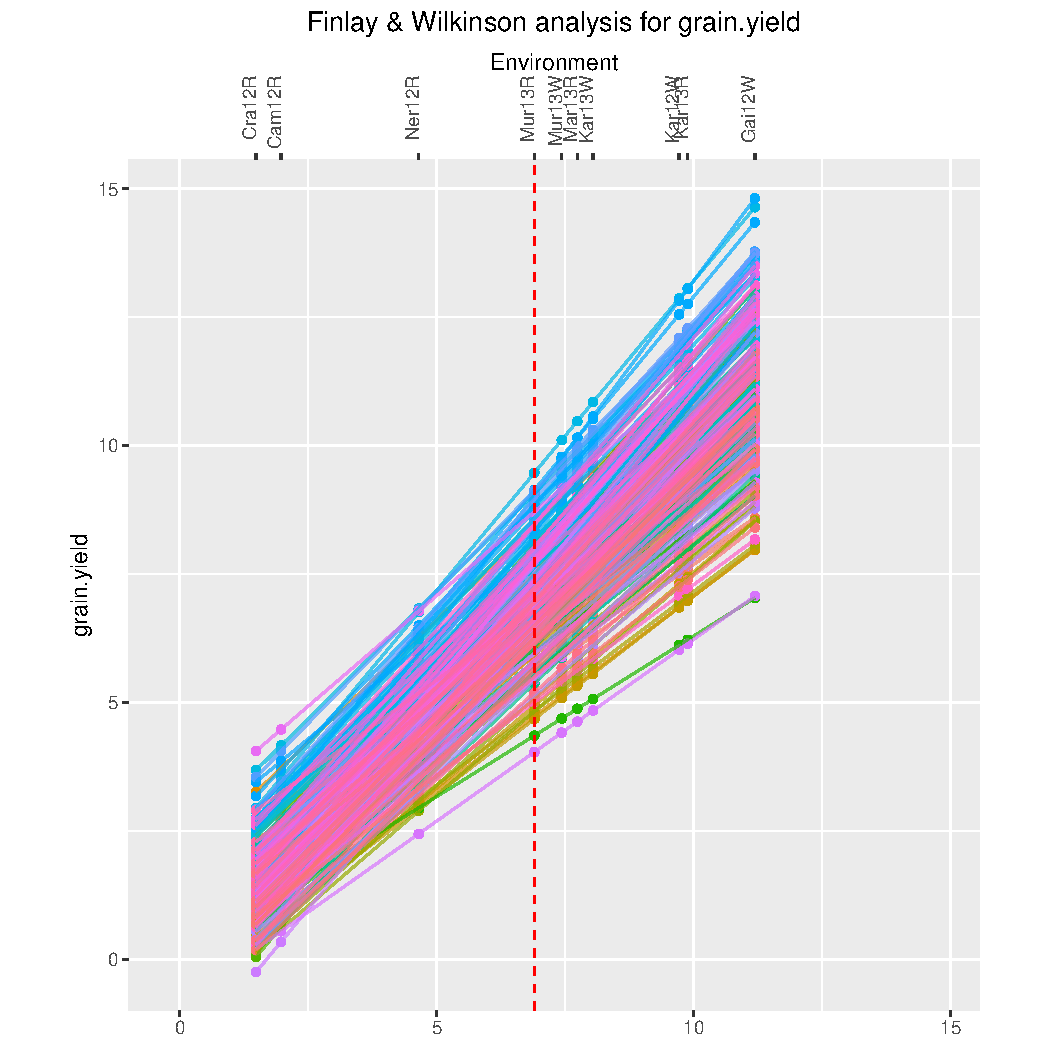
\includegraphics[width=0.9\linewidth]{./figures/112423080916-linePlot-1} \hfill{}


\end{knitrout}
\clearpage
\begin{knitrout}
\definecolor{shadecolor}{rgb}{0.969, 0.969, 0.969}\color{fgcolor}
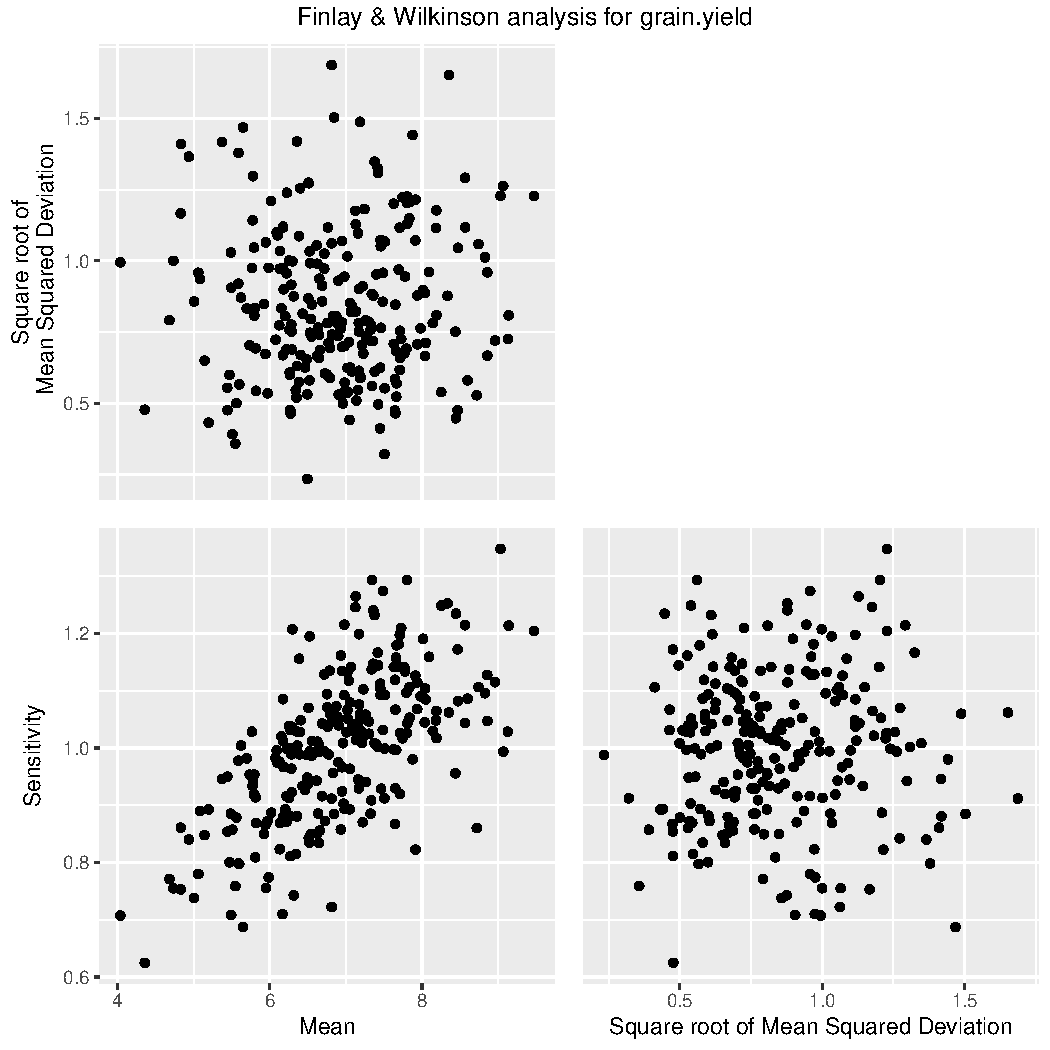
\includegraphics[width=0.9\linewidth]{./figures/112423080916-scatterPlot-1} 
\end{knitrout}
\clearpage

%-------------------------------------------------------------------------------
\section{Finlay-Wilkinson model parameter estimates}
%-------------------------------------------------------------------------------

\begin{kframe}


{\ttfamily\noindent\bfseries\color{errorcolor}{\#\# Error in order(estimates[[sortBy]], decreasing = TRUE): argument 1 is not a vector}}\end{kframe}% latex table generated in R 4.3.0 by xtable 1.8-4 package
% Fri Nov 24 08:09:18 2023
\begin{table}[ht]
\begin{flushleft}
\caption{Top 10 genotypes by sensitivity} 
\label{topEstimates}
\begin{tabular}{lrrrrrr}
  \hline
Genotype & GenMean & SE\_GenMean & Rank & Sens & SE\_Sens & MSdeviation \\ 
  \hline
Lo1251 & 9.03 & 0.28 & 1.00 & 1.35 & 0.09 & 1.51 \\ 
  DK78371A & 7.34 & 0.28 & 2.00 & 1.29 & 0.09 & 0.31 \\ 
  PHG83 & 7.80 & 0.28 & 3.00 & 1.29 & 0.09 & 1.45 \\ 
  FR697 & 7.49 & 0.28 & 4.00 & 1.27 & 0.09 & 0.92 \\ 
  SC-Malawi & 7.13 & 0.28 & 5.00 & 1.26 & 0.09 & 1.27 \\ 
  Lo1106 & 8.33 & 0.28 & 6.00 & 1.25 & 0.09 & 0.77 \\ 
  Lo1199 & 8.25 & 0.28 & 7.00 & 1.25 & 0.09 & 0.29 \\ 
  B98 & 7.12 & 0.28 & 8.00 & 1.25 & 0.09 & 1.38 \\ 
  DKMBST & 7.36 & 0.28 & 9.00 & 1.24 & 0.09 & 0.77 \\ 
  Lo904 & 8.44 & 0.28 & 10.00 & 1.23 & 0.09 & 0.20 \\ 
   \hline
\end{tabular}
\end{flushleft}
\end{table}
% latex table generated in R 4.3.0 by xtable 1.8-4 package
% Fri Nov 24 08:09:18 2023
\begin{table}[ht]
\begin{flushleft}
\caption{Bottom 10 genotypes by sensitivity} 
\label{bottomEstimates}
\begin{tabular}{lrrrrrr}
  \hline
Genotype & GenMean & SE\_GenMean & Rank & Sens & SE\_Sens & MSdeviation \\ 
  \hline
Os426 & 5.95 & 0.28 & 236.00 & 0.76 & 0.09 & 1.13 \\ 
  CO109 & 4.73 & 0.28 & 237.00 & 0.75 & 0.09 & 1.00 \\ 
  EP10 & 4.83 & 0.28 & 238.00 & 0.75 & 0.09 & 1.36 \\ 
  N16 & 6.32 & 0.28 & 239.00 & 0.74 & 0.09 & 0.77 \\ 
  UH\_2500 & 5.01 & 0.28 & 240.00 & 0.74 & 0.09 & 0.73 \\ 
  UH\_P089 & 6.81 & 0.28 & 241.00 & 0.72 & 0.09 & 1.13 \\ 
  EC151 & 6.17 & 0.28 & 242.00 & 0.71 & 0.09 & 0.95 \\ 
  A347 & 5.49 & 0.28 & 243.00 & 0.71 & 0.09 & 0.82 \\ 
  Pa36 & 4.04 & 0.28 & 244.00 & 0.71 & 0.09 & 0.99 \\ 
  A310 & 5.65 & 0.28 & 245.00 & 0.69 & 0.09 & 2.16 \\ 
  F252 & 4.36 & 0.28 & 246.00 & 0.62 & 0.09 & 0.23 \\ 
   \hline
\end{tabular}
\end{flushleft}
\end{table}

%-------------------------------------------------------------------------------
% End Document
\end{document}
